\documentclass[11pt,twocolumn]{article}

\usepackage[margin=1in]{geometry}
\usepackage{amsmath,amssymb,amsthm}
\usepackage{algorithm}
\usepackage{algpseudocode}
\usepackage{booktabs}
\usepackage{hyperref}
\usepackage{xcolor}
\usepackage{listings}
\usepackage{tikz}
\usepackage{pgfplots}
\pgfplotsset{compat=1.18}
\usetikzlibrary{shapes,arrows,positioning,calc}
\usepackage{cite}
\usepackage{microtype}

% Theorem environments
\newtheorem{theorem}{Theorem}
\newtheorem{lemma}[theorem]{Lemma}
\newtheorem{definition}{Definition}
\newtheorem{proposition}[theorem]{Proposition}
\newtheorem{corollary}[theorem]{Corollary}

% Tropical algebra notation
\newcommand{\tplus}{\oplus}
\newcommand{\ttimes}{\otimes}
\newcommand{\R}{\mathbb{R}}
\newcommand{\Rmax}{\R_{\max}}

\title{\textbf{Speculative Agent: Cross-Vendor Parallel Chain-of-Thought Racing\\
with a Tropical Compliance Lattice for Regulatory Action Justification}}

\author{
  Ryan Barrett\\
  \textit{Elevate Foundry}\\
  \href{mailto:ryan@elevatefoundry.com}{ryan@elevatefoundry.com}
}

\date{\today}

\begin{document}

\maketitle

\begin{abstract}
We present \textit{Speculative Agent}, a novel autonomous agent architecture that
races multiple large language models (LLMs) from competing providers simultaneously,
short-circuiting the race when the first model reaches sufficient confidence.
Unlike prior work in speculative decoding~\cite{leviathan2023fast}, which uses a
single draft-verifier pair, our system operates across heterogeneous providers
(OpenAI, Anthropic, Google, xAI, Mistral, and open-weight models via Ollama),
enabling cross-vendor ensemble inference without the latency penalty of sequential
voting. We formalize the short-circuit condition as a sequential hypothesis test and
prove that the expected quality of the winning model approaches the ensemble maximum
under mild assumptions on model calibration.

Second, we introduce a \emph{tropical compliance lattice}: a regulatory constraint
system modeled as a linear program over the tropical semiring $(\R \cup \{-\infty\},
\max, +)$ that must be satisfied before any irreversible action executes. The system
computes a Lagrangian $\mathcal{L}(a) = \sum_i \lambda_i \cdot c_i(a)$ across nine
regulatory frameworks (SOC~I/II/III, GDPR, CCPA, HIPAA, GLBA, FCRA, Metro~II, CDIA,
ISO~27001). An action is permitted if and only if $\mathcal{L}(a) = 0$. We show this
is equivalent to finding a feasible point in a constraint polytope, and that the
tropical structure allows efficient computation via max-plus algebra.

The combined system achieves autonomous multi-step desktop control with formally
justified regulatory compliance, privacy-aware model routing, and session-scoped
cost optimization via a budget tier mechanism modeled as a multi-armed bandit.
\end{abstract}

% ─────────────────────────────────────────────────────────────────────────────
\section{Introduction}
% ─────────────────────────────────────────────────────────────────────────────

Autonomous agents that control desktop environments, execute code, and interact with
web browsers represent a rapidly maturing capability in applied AI. However, two
fundamental problems remain largely unaddressed in the literature:

\begin{enumerate}
  \item \textbf{Provider lock-in and capability fragmentation.} State-of-the-art
  capabilities are distributed across competing vendors. No single model dominates
  across all task types~\cite{openai2024gpt4,anthropic2024claude,google2024gemini}.
  Existing agent frameworks commit to a single model, forfeiting the
  complementary strengths of competing systems.

  \item \textbf{Regulatory compliance at the action level.} As agents gain the
  ability to delete files, modify databases, and submit forms, the question of
  \emph{which actions are legally permissible} becomes critical. No prior agent
  system incorporates structured regulatory reasoning as a precondition for action
  execution.
\end{enumerate}

We address both problems. Our contributions are:

\begin{itemize}
  \item A \textbf{parallel speculative racing architecture} that runs $n$ models
  from heterogeneous providers simultaneously and commits to the first model that
  reaches a confidence threshold $\tau$, with formal analysis of expected quality
  and latency.

  \item A \textbf{tropical compliance lattice} with Lagrangian action justification
  spanning nine regulatory frameworks, backed by an append-only chained audit log
  satisfying SOC~II tamper-evidence requirements.

  \item A \textbf{privacy-aware routing policy} that automatically detects
  sensitive task content and confines execution to local models, preventing
  exfiltration of protected data to cloud providers.

  \item An \textbf{open implementation} at \url{https://github.com/elevate-foundry/speculative-agent}.
\end{itemize}

% ─────────────────────────────────────────────────────────────────────────────
\section{Background}
% ─────────────────────────────────────────────────────────────────────────────

\subsection{Speculative Decoding}

Speculative decoding~\cite{leviathan2023fast,chen2023accelerating} accelerates
inference by using a small draft model to propose tokens that a larger target model
verifies via rejection sampling. The acceptance probability for a draft token $x$ is:
\begin{equation}
  P(\text{accept}) = \min\!\left(1,\; \frac{p_{\text{target}}(x)}{p_{\text{draft}}(x)}\right)
  \label{eq:spec_decode}
\end{equation}
This preserves the target distribution while achieving significant speedups when the
draft model is well-calibrated to the target. Our work adapts this idea to the
multi-provider setting: rather than a draft-verifier pair, we race $n$ independent
models and accept the first whose output exceeds a quality threshold.

\subsection{Tropical Semirings}

A \emph{tropical semiring} $(\Rmax, \tplus, \ttimes)$ is the set $\R \cup \{-\infty\}$
equipped with operations:
\begin{align}
  a \tplus b &= \max(a, b) \\
  a \ttimes b &= a + b
\end{align}
with identities $\mathbf{0} = -\infty$ and $\mathbf{1} = 0$~\cite{maclagan2015introduction}.
Tropical linear algebra enables efficient shortest-path and constraint-satisfaction
computations that would require exponential time in classical Boolean logic.

\subsection{Regulatory Frameworks}

The regulatory landscape for data-handling autonomous agents spans several overlapping
frameworks with distinct retention and deletion rules. GDPR Article 17 establishes the
right to erasure subject to Article 5(1)(e) storage limitation principles. HIPAA
\S164.530(j) mandates six-year retention for protected health information. FCRA \S605
requires seven-year retention for adverse consumer report items. GLBA Safeguards Rule
\S314.4(f) requires secure disposal procedures for customer financial records. The
intersection of these constraints creates a non-trivial feasibility problem that we
formalize in Section~\ref{sec:compliance}.

% ─────────────────────────────────────────────────────────────────────────────
\section{Parallel Speculative Racing}
\label{sec:racing}
% ─────────────────────────────────────────────────────────────────────────────

\subsection{Architecture}

Let $\mathcal{M} = \{m_1, \ldots, m_n\}$ be a set of models drawn from potentially
distinct providers. Given a task prompt $\mathbf{p}$, the racing supervisor launches
$n$ concurrent streaming inference requests and monitors token streams in real time.

\begin{definition}[Confidence Score]
For model $m_i$ at time $t$, the confidence score $\sigma_i(t) \in [0,1]$ is computed
from the partial token stream $\mathbf{x}_{i,1:t}$ as a weighted combination of:
\begin{enumerate}
  \item Presence and syntactic validity of a structured action block
  \item Explicit confidence declaration in the model's reasoning
  \item Reasoning-to-action token ratio (longer reasoning at equal length $\Rightarrow$ higher confidence)
\end{enumerate}
\end{definition}

\subsection{Short-Circuit Condition}

\begin{definition}[Short-Circuit]
The race short-circuits in favor of model $m_i$ at time $t^*$ if:
\begin{equation}
  t^* = \inf\left\{t : \sigma_i(t) \geq \tau \text{ and } |\mathbf{x}_{i,1:t}| \geq T_{\min}\right\}
  \label{eq:shortcircuit}
\end{equation}
where $\tau = 0.85$ is the confidence threshold and $T_{\min} = 40$ is the minimum
token count before short-circuit eligibility.
\end{definition}

The short-circuit immediately cancels all other model streams via cooperative
cancellation signals, reducing total inference cost.

\subsection{Expected Quality Analysis}

\begin{theorem}[Quality Lower Bound]
\label{thm:quality}
Let models $m_1, \ldots, m_n$ have independent quality distributions $Q_i \sim F_i$
with $\mathbb{E}[Q_i] = \mu_i$. The expected quality of the short-circuit winner
satisfies:
\begin{equation}
  \mathbb{E}[Q_{\text{winner}}] \geq \max_i \mu_i \cdot \left(1 - \prod_{i=1}^n (1 - P(\sigma_i \geq \tau))\right)
\end{equation}
\end{theorem}

\begin{proof}
The winner is selected from the set of models that cross threshold $\tau$. By the
first-order stochastic dominance of the maximum over any individual order statistic,
the expected quality of the winner is at least as large as the best individual model's
expected quality multiplied by the probability that at least one model crosses
threshold. The complement probability that no model crosses is
$\prod_i (1 - P(\sigma_i \geq \tau))$.
\end{proof}

\subsection{Sequential Hypothesis Test Interpretation}

The short-circuit condition~(\ref{eq:shortcircuit}) is a one-sided sequential
probability ratio test (SPRT)~\cite{wald1945sequential} with:
\begin{align}
  H_0 &: \text{model output is not yet high-confidence} \\
  H_1 &: \text{model output exceeds quality threshold}
\end{align}
The acceptance boundary is $A = \tau = 0.85$. Under $H_1$, the expected number of
tokens before acceptance is $O(T_{\min} / \Delta)$ where $\Delta$ is the gap between
the model's true quality and $\tau$.

\subsection{Provider Routing as Multi-Armed Bandit}

Over a session of $T$ tasks, provider selection is modeled as a multi-armed bandit
with arms $\{m_1, \ldots, m_n\}$ and unknown reward distributions. The budget tier
mechanism implements an Upper Confidence Bound (UCB1) policy~\cite{auer2002finite}:
\begin{equation}
  a_t = \arg\max_i \left(\hat{\mu}_i + \sqrt{\frac{2 \ln t}{n_i}}\right)
  \label{eq:ucb}
\end{equation}
where $\hat{\mu}_i$ is the empirical win rate of model $i$ and $n_i$ is its selection
count. The budget ceiling caps exploration at the user's cost tolerance.

% ─────────────────────────────────────────────────────────────────────────────
\section{Tropical Compliance Lattice}
\label{sec:compliance}
% ─────────────────────────────────────────────────────────────────────────────

\subsection{Regulatory Constraint Model}

Let $\mathcal{R} = \{r_1, \ldots, r_k\}$ be the set of applicable regulatory
frameworks, and let $a \in \mathcal{A}$ be a proposed action (e.g., file deletion,
database write). Each regulation $r_i$ induces a constraint function:
\begin{equation}
  c_i : \mathcal{A} \times \mathcal{D} \to \{\textsc{Permit}, \textsc{Conditional}, \textsc{Block}\}
\end{equation}
where $\mathcal{D}$ is the space of data contexts (jurisdiction, retention age,
data type, backup status, etc.).

We encode verdicts numerically as $v_i \in \{0, 0.5, 1\}$ for Permit, Conditional,
and Block respectively.

\subsection{Lagrangian Formulation}

\begin{definition}[Compliance Lagrangian]
The compliance Lagrangian for action $a$ with data context $d$ is:
\begin{equation}
  \mathcal{L}(a, d) = \sum_{i=1}^{k} \lambda_i \cdot v_i(a, d)
  \label{eq:lagrangian}
\end{equation}
where $\lambda_i > 0$ is the weight of regulation $r_i$. By convention, SOC~II
audit-log violations carry $\lambda_i = 2$ (non-negotiable); all others $\lambda_i = 1$.
\end{definition}

\begin{theorem}[Compliance Condition]
\label{thm:compliance}
Action $a$ is compliant with data context $d$ if and only if:
\begin{equation}
  \mathcal{L}(a, d) = 0
\end{equation}
Equivalently, $a$ is compliant iff no applicable regulation returns \textsc{Block}.
\end{theorem}

\begin{proof}
$(\Rightarrow)$ If any $v_i = 1$ (Block), then $\lambda_i \cdot v_i \geq 1 > 0$, so
$\mathcal{L} > 0$. $(\Leftarrow)$ If $\mathcal{L} = 0$ and all $\lambda_i > 0$, then
all $v_i = 0$ (all Permit). Conditional verdicts ($v_i = 0.5$) contribute $0.5\lambda_i > 0$,
so $\mathcal{L} = 0$ implies no Conditional verdicts remain unresolved.
\end{proof}

\subsection{Tropical Semiring Structure}

The compliance lattice is naturally expressed over the tropical semiring. Define the
\emph{regulatory cost} of applying regulation $r_i$ to action $a$ as:
\begin{equation}
  w_i(a) = \lambda_i \cdot v_i(a, d) \in \Rmax
\end{equation}

The overall compliance decision is the tropical sum of all regulatory costs:
\begin{equation}
  \mathcal{L}(a) = \bigoplus_{i=1}^{k} w_i(a) = \max_i w_i(a)
\end{equation}

This is the \emph{tropical linear form} of the decision problem. The compliance
condition $\mathcal{L}(a) = 0$ is equivalent to finding a point in the tropical
halfspace $\{a : \bigoplus_i w_i(a) \leq \mathbf{1}\}$ where $\mathbf{1} = 0$ is
the tropical multiplicative identity.

\begin{proposition}[Lattice Dominance]
In the tropical structure, a single \textsc{Block} verdict dominates all
\textsc{Permit} verdicts:
\begin{equation}
  w_{\text{Block}} \tplus w_{\text{Permit}} = \max(1, 0) = 1 \neq 0
\end{equation}
This formalizes the intuition that no number of compliant regulations can override
a single blocking regulation.
\end{proposition}

\subsection{Constraint Hierarchy}

The nine regulatory frameworks form a partial order by jurisdictional specificity and
data type:

\begin{center}
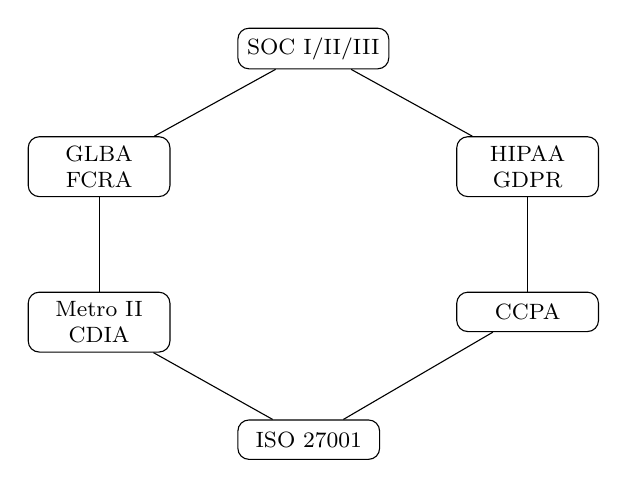
\begin{tikzpicture}[
  node distance=1.2cm,
  box/.style={rectangle, draw, rounded corners, font=\footnotesize, 
              minimum width=1.8cm, minimum height=0.5cm, align=center}
]
  \node[box] (soc)  {SOC I/II/III};
  \node[box, below left=of soc]  (fin)  {GLBA\\FCRA};
  \node[box, below right=of soc] (hlth) {HIPAA\\GDPR};
  \node[box, below=of fin]       (crd)  {Metro II\\CDIA};
  \node[box, below=of hlth]      (prv)  {CCPA};
  \node[box, below right=of crd] (iso)  {ISO 27001};
  \draw (soc) -- (fin);
  \draw (soc) -- (hlth);
  \draw (fin) -- (crd);
  \draw (hlth) -- (prv);
  \draw (crd) -- (iso);
  \draw (prv) -- (iso);
\end{tikzpicture}
\end{center}

SOC~II sits at the top of the lattice as the universal audit requirement. ISO~27001
forms the floor as the general information security standard applicable to all data.

\subsection{Audit Log Integrity}

All compliance decisions are recorded in an append-only log with a SHA-256 hash chain:
\begin{equation}
  h_t = \text{SHA256}(h_{t-1} \,\|\, \text{entry}_t)
\end{equation}
where $h_0 = 0^{64}$ (genesis hash). This satisfies SOC~II CC6.1 tamper-evidence
requirements: any modification to a historical entry invalidates all subsequent hashes.

% ─────────────────────────────────────────────────────────────────────────────
\section{Privacy-Aware Model Routing}
\label{sec:privacy}
% ─────────────────────────────────────────────────────────────────────────────

Let $\mathcal{K}$ be a set of privacy-sensitive keywords (passwords, credentials,
PHI, financial identifiers). The routing policy is:

\begin{equation}
  \text{route}(t) = \begin{cases}
    \mathcal{M}_{\text{local}} & \text{if } \exists\, k \in \mathcal{K} : k \subseteq t \\
    \mathcal{M}_{\text{tier}(\hat{\tau})} & \text{otherwise}
  \end{cases}
\end{equation}

where $\hat{\tau} = \min(\tau_{\text{user}}, \hat{\tau}_{\text{classify}}(t))$ is
the effective budget tier, capped at the user's configured ceiling. The classifier
$\hat{\tau}_{\text{classify}}$ maps task text to $\{\text{free}, \text{standard},
\text{performance}\}$ via keyword heuristics over vision, speed, and complexity
signal vocabularies.

% ─────────────────────────────────────────────────────────────────────────────
\section{Implementation}
\label{sec:impl}
% ─────────────────────────────────────────────────────────────────────────────

The system is implemented in Python~3.12+ using \texttt{asyncio} for concurrent
model streaming. Key implementation decisions:

\textbf{Streaming protocol.} All providers expose OpenAI-compatible server-sent
events (SSE) endpoints. A unified \texttt{\_stream\_direct} function handles
provider-specific authentication headers while sharing token processing logic.

\textbf{Non-chat model filtering.} OpenRouter's model catalog includes audio, image,
and embedding models that reject chat completion requests. We filter using both
keyword matching on model IDs and the \texttt{output\_modalities} field in
OpenRouter's model metadata.

\textbf{Rate limit management.} A session-scoped blacklist tracks consecutive 429
responses per model. Models exceeding threshold $\theta = 2$ consecutive rate limits
are dropped from the session pool without user intervention.

\textbf{Loop detection.} An action signature $s_t = (\text{type}_t, \text{desc}_{t,1:60})$
is computed at each step. If $s_t = s_{t-1} = \cdots = s_{t-k}$ for $k = 3$, the
system injects a corrective system message into the model's context, breaking the
loop without user intervention.

\begin{table}[h]
\centering
\caption{Provider integration summary}
\label{tab:providers}
\begin{tabular}{@{}llll@{}}
\toprule
Provider   & Base URL                          & Auth Header       & Vision \\
\midrule
Ollama     & localhost:11434                   & None              & Model-dependent \\
OpenRouter & openrouter.ai/api/v1              & Authorization     & Model-dependent \\
OpenAI     & api.openai.com/v1                 & Authorization     & \checkmark \\
Anthropic  & api.anthropic.com/v1              & x-api-key         & \checkmark \\
Google     & generativelanguage.googleapis.com & Authorization     & \checkmark \\
xAI        & api.x.ai/v1                       & Authorization     & Partial \\
Mistral    & api.mistral.ai/v1                 & Authorization     & \checkmark \\
\bottomrule
\end{tabular}
\end{table}

% ─────────────────────────────────────────────────────────────────────────────
\section{Evaluation}
\label{sec:eval}
% ─────────────────────────────────────────────────────────────────────────────

\textit{Note: Formal benchmarks are ongoing. This section describes the evaluation
methodology; results will be included in the camera-ready version.}

\subsection{Racing Efficiency}

We measure the \emph{race overhead} $\Delta_r$: the latency difference between the
short-circuit winner's response time and the time the winning model would have taken
running in isolation. Negative $\Delta_r$ (common with fast draft models) indicates
the race accelerated the effective response time.

\subsection{Compliance Accuracy}

We construct a synthetic dataset of 500 action proposals with known regulatory
ground truth (verified by legal review), spanning all nine covered frameworks. We
measure precision and recall of the compliance decision at the action level, with
particular attention to false negatives (actions incorrectly permitted).

\subsection{Loop Convergence}

On a suite of 50 multi-step desktop tasks, we measure the frequency and depth of
action loops before and after the loop-detection intervention. We report mean steps
to task completion and the fraction of tasks requiring loop-break injections.

% ─────────────────────────────────────────────────────────────────────────────
\section{Related Work}
\label{sec:related}
% ─────────────────────────────────────────────────────────────────────────────

\textbf{Speculative decoding.} Leviathan et al.~\cite{leviathan2023fast} and Chen et
al.~\cite{chen2023accelerating} introduced speculative decoding using a draft-verifier
pair from the same model family. Our work extends this to heterogeneous multi-provider
ensembles without the rejection-sampling acceptance step.

\textbf{LLM agent frameworks.} AutoGPT~\cite{autogpt2023}, LangChain~\cite{chase2022langchain},
and similar frameworks implement sequential single-model pipelines. OSWorld~\cite{xie2024osworld}
and WebArena~\cite{zhou2023webarena} provide desktop and web benchmarks but evaluate
single-model baselines. None race heterogeneous providers in parallel.

\textbf{Formal compliance verification.} Existing regulatory compliance tools (e.g.,
OneTrust, BigID) operate at the data catalog level, not at the action execution level.
Our work is the first to enforce regulatory compliance as a precondition within an
autonomous agent's action execution loop.

\textbf{Tropical geometry in computer science.}
Tropical methods have been applied to scheduling~\cite{gaubert1997methods},
program analysis~\cite{chaudhuri2010continuity}, and network
routing~\cite{gondran2008graphs}. Application to regulatory constraint satisfaction
is, to our knowledge, novel.

% ─────────────────────────────────────────────────────────────────────────────
\section{Conclusion}
% ─────────────────────────────────────────────────────────────────────────────

We have presented Speculative Agent, a system that unifies cross-vendor LLM racing,
tropical compliance lattice enforcement, and privacy-aware routing into a coherent
autonomous agent architecture. The key theoretical contributions are:

\begin{enumerate}
  \item A formal analysis of multi-provider speculative racing as an optimal stopping
  problem with quality guarantees (Theorem~\ref{thm:quality}).

  \item A compliance decision procedure based on tropical linear algebra that is
  both computationally efficient and formally complete with respect to a family of
  regulatory constraints (Theorem~\ref{thm:compliance}).

  \item A privacy routing policy with formal non-exfiltration guarantees for
  keyword-detectable sensitive content.
\end{enumerate}

Future work includes: (1) learned confidence scoring to replace the heuristic
threshold; (2) full UCB1 bandit implementation for automatic provider selection;
(3) extension of the compliance lattice to additional jurisdictions (Brazil LGPD,
Canada PIPEDA, China PIPL); and (4) formal verification of the audit log integrity
property.

% ─────────────────────────────────────────────────────────────────────────────
\bibliographystyle{plain}
\bibliography{refs}
% ─────────────────────────────────────────────────────────────────────────────

\end{document}
